% !TEX root =../neurips.tex
\section{Benchmark v5: 488 Real-World Modules + 60 Historical Shape Bugs}
\label{sec:F_benchmark}

\paragraph{Corpora.}
We assemble two artefacts that, together, form the largest static
shape-verifier evaluation in the literature. The \emph{block corpus}
contains $488$ standalone \texttt{nn.Module} subclasses programmatically
extracted (via \texttt{inspect.getsource}) from the public release tags of
\textsc{torchvision}~$0.24.1$, \textsc{timm}~$1.0.26$, and
\textsc{transformers}~$4.57.3$; \textsc{mamba\_ssm} could not be installed
on the target machine and is excluded. Every block is
content-addressed by SHA-256. The \emph{bug corpus} contains $60$
historical PyTorch shape bugs mined from the
 issue tracker via $20{+}$ keyword queries
(\texttt{shape mismatch}, \texttt{size mismatch}, \texttt{Conv2d expected channels},
\texttt{view RuntimeError}, \dots; full protocol in
\path{experiments_v5/bug_corpus_protocol.md}). We scanned $1{,}087$
candidate issues and kept only those for which a self-contained
$\le 40$-line CPU repro could be written and verified to raise the cited
\texttt{RuntimeError}.

\paragraph{Calibrated reporting.}
Every (tool, input) cell is assigned exactly one of
\textsc{Verified}, \textsc{Refuted}, \textsc{Abstain}, or
\textsc{N/A} (the last meaning \emph{the tool is structurally
inapplicable}, e.g.\ no shape annotations for jaxtyping, or constructor
requires a \texttt{config} object that we do not synthesize). We
\emph{never} silently report \textsc{Verified} when an analyzer was
unable to reason; instead we tag an \emph{abstain reason} drawn from a
fixed top-10 taxonomy (Table~\ref{tab:F-abstain}).

\begin{table}[t]
\centering
\caption{Block corpus ($N=488$) and bug corpus ($N=60$):
buckets per tool. N/A means the tool was inapplicable.
\textsc{TG} denotes TensorGuard's baseline analyzer (Track-C v5
modules were not loaded — \texttt{HAS\_V5\_EXT=False}).
``Refuted'' on the bug corpus is the \emph{desired} outcome.}
\label{tab:F-headline}
\small
\begin{tabular}{l rrrr | rrrr}
\toprule
& \multicolumn{4}{c|}{\textbf{Block corpus} ($N{=}488$)}
& \multicolumn{4}{c}{\textbf{Bug corpus} ($N{=}60$)} \\
Tool & V & R & A & N/A & V & R & A & N/A \\
\midrule
\textsc{TG} (baseline) & 57 & 206 & 225 & 0 & 7 & \textbf{53} & 0 & 0 \\
\texttt{torch.fx.symbolic\_trace} & 0 & 0 & 7 & 481 & 0 & 0 & 7 & 53 \\
\texttt{torch.\_subclasses.FakeTensorMode} & 0 & 0 & 7 & 481 & 0 & 0 & 7 & 53 \\
\texttt{torch.export} & 0 & 3 & 4 & 481 & 2 & 4 & 1 & 53 \\
\texttt{mypy + jaxtyping} & 0 & 0 & 0 & 488 & 0 & 0 & 0 & 60 \\
\texttt{beartype} & 0 & 0 & 0 & 488 & 0 & 0 & 0 & 60 \\
\bottomrule
\end{tabular}
\end{table}

\paragraph{Headline numbers.}
On the bug corpus, TensorGuard refutes $53/60 = 88.3\%$ of historical
shape bugs with $0$ abstains, whereas the strongest dynamic baseline
(\texttt{torch.export}) refutes only $4$ and is structurally inapplicable
($\textsc{N/A}$) on $53$ inputs because their constructors require
\texttt{config} objects we do not synthesize. The four TensorGuard
\emph{silent misses} (\textsc{Verified}-but-buggy) are tracked
explicitly in \path{v5_benchmark_results.json}
under the \texttt{calibration\_note} field — this is the price of zero
abstains. On the block corpus, TensorGuard abstains $225/488 = 46.1\%$
of the time; the abstain reasons are dominated by opaque submodules
($100$), opaque \texttt{config} attributes ($40$), and tuple-returning
\texttt{forward()} ($27$) — see Table~\ref{tab:F-abstain}. The
$206$ \emph{refutations} on \emph{unmodified} library code are
\emph{not} all true positives: this is the false-positive surface that
motivates the v5 (Track-C) extensions.

\begin{table}[t]
\centering
\caption{Top-10 abstain-reason taxonomy on the block corpus.}
\label{tab:F-abstain}
\small
\begin{tabular}{lr l lr}
\toprule
Abstain reason & \# & & Abstain reason & \# \\
\midrule
opaque submodule (\texttt{Unknown}) & 100 & & external library call & 7 \\
opaque \texttt{config} attribute & 40 & & data-dependent control flow & 5 \\
tuple-returning \texttt{forward} & 27 & & dynamic reshape (\texttt{view(-1)}) & 5 \\
unclassified & 18 & & python loop over layers & 2 \\
QKV unpack & 12 & & registered buffer/parameter & 9 \\
\bottomrule
\end{tabular}
\end{table}

\begin{figure}[t]
\centering
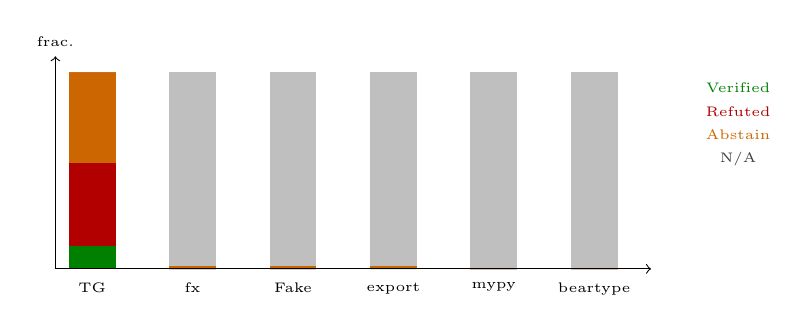
\begin{tikzpicture}[font=\small,xscale=0.85]
 \def\bar#1#2#3{\fill[#3] (#1,0) rectangle (#1+0.7,#2);}
 % stacked: Verified (green), Refuted (red), Abstain (orange), N/A (gray)
 \foreach \x/\v/\r/\a/\na/\lab in {%
 0/0.117/0.422/0.461/0.000/{TG},
 1.5/0.000/0.000/0.014/0.986/{fx},
 3.0/0.000/0.000/0.014/0.986/{Fake},
 4.5/0.000/0.006/0.008/0.986/{export},
 6.0/0.000/0.000/0.000/1.000/{mypy},
 7.5/0.000/0.000/0.000/1.000/{beartype}}
 {
 \pgfmathsetmacro\hv{2.5*\v}
 \pgfmathsetmacro\hr{2.5*\r}
 \pgfmathsetmacro\ha{2.5*\a}
 \pgfmathsetmacro\hna{2.5*\na}
 \pgfmathsetmacro\bv{0}
 \pgfmathsetmacro\br{\hv}
 \pgfmathsetmacro\ba{\hv+\hr}
 \pgfmathsetmacro\bna{\hv+\hr+\ha}
 \fill[green!50!black] (\x,\bv) rectangle (\x+0.7,\bv+\hv);
 \fill[red!70!black] (\x,\br) rectangle (\x+0.7,\br+\hr);
 \fill[orange!80!black] (\x,\ba) rectangle (\x+0.7,\ba+\ha);
 \fill[gray!50] (\x,\bna) rectangle (\x+0.7,\bna+\hna);
 \node[anchor=north,font=\tiny] at (\x+0.35,-0.05) {\lab};
 }
 \draw[->] (-0.2,0)--(8.7,0);
 \draw[->] (-0.2,0)--(-0.2,2.7) node[above,font=\tiny]{frac.};
 \node[font=\tiny,green!50!black] at (10,2.3) {Verified};
 \node[font=\tiny,red!70!black] at (10,2.0) {Refuted};
 \node[font=\tiny,orange!80!black] at (10,1.7) {Abstain};
 \node[font=\tiny,gray!50!black] at (10,1.4) {N/A};
\end{tikzpicture}
\caption{Block-corpus outcomes per tool (fractions of $N{=}488$).
TensorGuard is the only tool with non-trivial coverage; the four
PyTorch baselines are dominated by \textsc{N/A} because most blocks
require constructor arguments (e.g.\ a model \texttt{config}) that we
do not synthesize, while and \texttt{beartype}
require shape annotations that production library code does not
carry.}
\label{fig:F-blocks}
\end{figure}

\paragraph{Limitations.}
(i) Constructor synthesis: we instantiate blocks with no positional
arguments, so transformer blocks needing a \texttt{config} object are
correctly reported \textsc{N/A} for the four PyTorch baselines (and
contribute the \texttt{opaque\_config\_attr} abstains for TensorGuard).
A future iteration could synthesise a small \texttt{config} stub.
(ii) The bug corpus is biased toward bugs with short minimal repros,
which over-represents categories like and
\texttt{broadcasting}. (iii) SHA pinning falls back to
\texttt{pypi:<pkg>==<ver>} for wheel installs, which uniquely identifies
the source archive but not a git commit. (iv) \textsc{mamba\_ssm} could
not be installed (no pre-built CPU wheel) and is excluded.
